\documentclass{beamer}
\usepackage[spanish]{babel}
\usepackage{tikz} 
\usepackage{tikz-network}
\usepackage[utf8]{inputenc}
\usepackage{hyperref}
\usepackage{algorithm,algorithmic}
\usetheme{CambridgeUS}
\usepackage{enumerate}
\usepackage{natbib}
\title[UQRSPFS]{Uso de Q-learning como alternativa a la solución del problema de programación de taller de trabajo flexible}
\author{Lic. Arnoldo Del Toro Peña }
\institute[UANL]{Universidad Autónoma de Nuevo León}
\newcommand{\fjssp}{problema de programación de taller de trabajo flexible}
\begin{document}

\begin{frame}
 \titlepage
\end{frame}

\begin{frame}{Introducción}
    \centering Modelos.

    \begin{figure}[h!t]
    \centering
    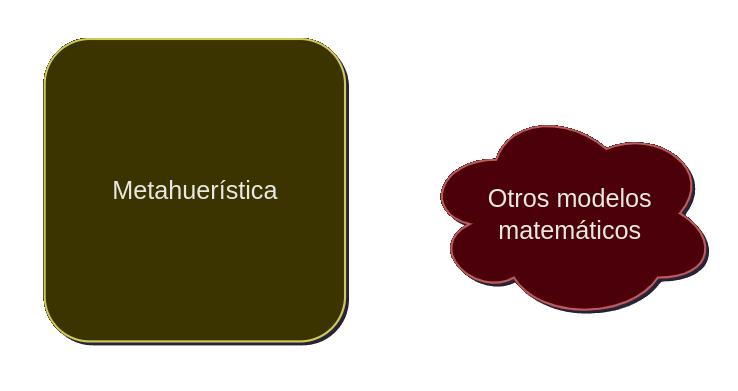
\includegraphics[scale = 0.4 ]{imagen1.png}
    %\caption{}
    %\label{}
    \end{figure}
    
\end{frame}

\begin{frame}{Introducción}{Objetivos}
\begin{block}<1->{}
    ¿Es viable utilizar la búsqueda aprendizaje por refuerzo (Q-learning) en el problema
de programación de taller de trabajo flexible?
\end{block}
\begin{block}<2->{}
	¿Bajo que
condiciones es favorable utilizar una búsqueda aprendizaje por refuerzo (Q-learning)?
\end{block}
\begin{figure}
	
\includegraphics[scale = 0.5]{preguntas}
\end{figure}
\end{frame}

\begin{frame}{Problema de programación de taller de trabajo flexible}
    \begin{block}<1->{}
        \centering
        \begin{figure}[h!t]
        \centering
        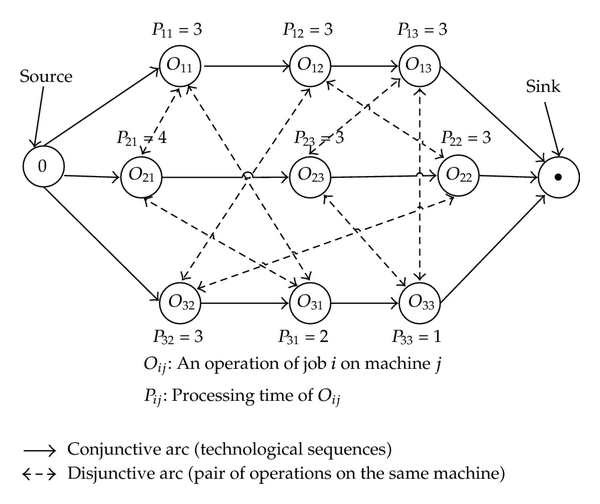
\includegraphics[scale = 1.25 ]{imagen3.jpg}
        %\caption{}
        %\label{}
        \end{figure}
    \end{block}
\end{frame}

\begin{frame}{Introducción}
\begin{figure}[h!t]
\centering
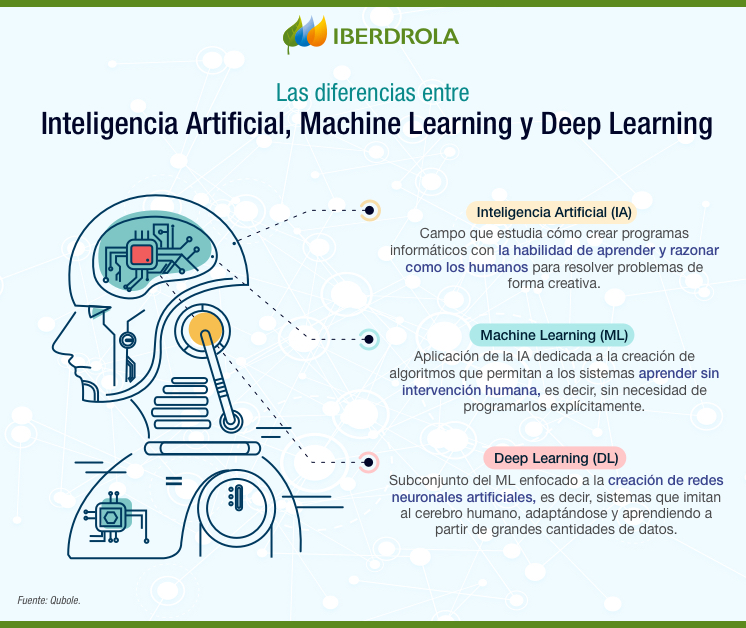
\includegraphics[scale = 1 ]{Deep_Learning_ESP.png}
%\label{}
\end{figure}
\end{frame}

\begin{frame}{Obstáculo}
    Tiempo y recursos.
        \begin{figure}[h!t]
        \centering
        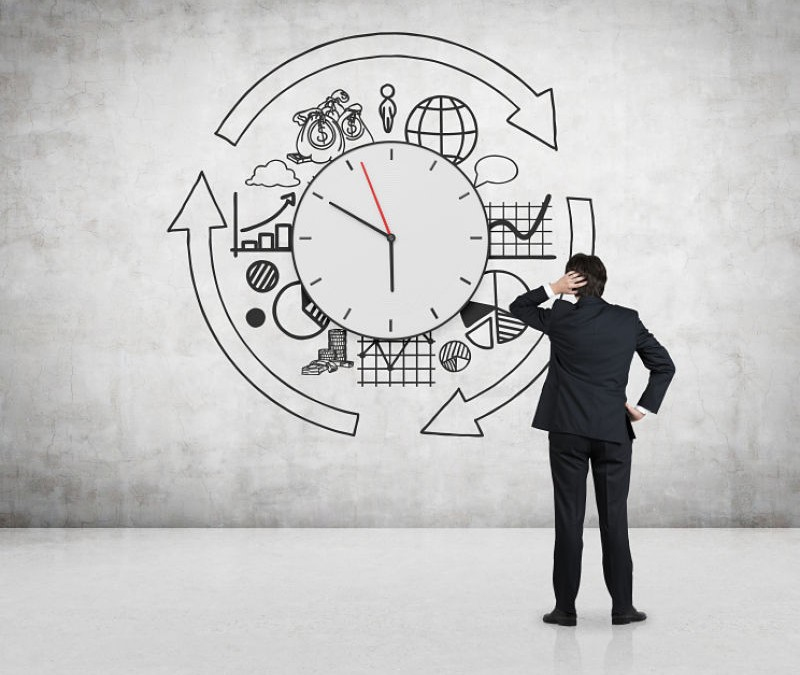
\includegraphics[scale = 0.25 ]{imagen4.jpg}
        %\caption{}
        %\label{}
        \end{figure}
\end{frame}

{
\setbeamertemplate{background} 
{
    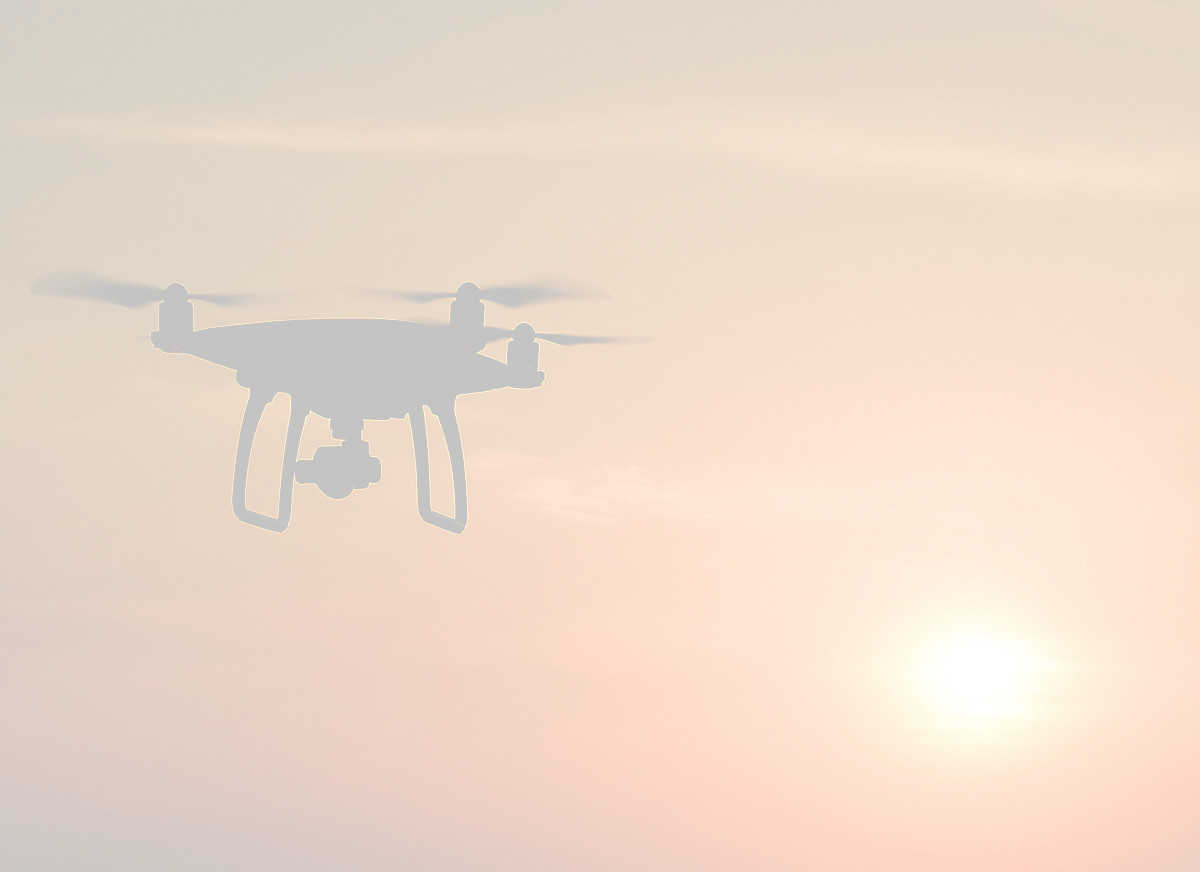
\includegraphics[width=\paperwidth,height=\paperheight]{imagen7.jpeg}
}
\begin{frame}{Antecedentes}

    {\centering \color{black} \citet{CHEN2022939} usan el aprendizaje por refuerzo (Q-learning) en un problema de entrega el mismo día (Same-day delivery) utilizando vehículos y drones, también detallan una solución aproximada usando el aprendizaje por refuerzo (Q-learning). }

\end{frame}
}

\begin{frame}{}
\centering  \cite{HUANG2022108353} presentan el método clasificación de corte (Cut Ranking) para seleccionar los cortes en un problema de ramificación y corte para programación entera mixta (mixed-integer programming).

\begin{figure}
	\centering
	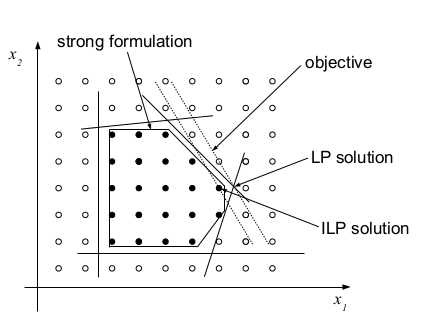
\includegraphics[scale = 0.4]{MIP}
\end{figure}

\end{frame}

\begin{frame}{}
	\cite{zhao2019improved} proponen la implementación de un algoritmo de doble capa de aprendizaje por refuerzo (Q-learning) así como acciones para la solución del problema dinámico de programación de talleres flexibles con fallas en máquinas.
\end{frame}

\begin{frame}{Metodología}

    \begin{figure}[h!t]
    \centering
    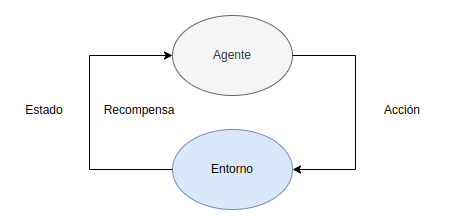
\includegraphics[scale = 0.7 ]{diagrama}
    %\caption{}
    %\label{}
    \end{figure}

\end{frame}

\begin{frame}{Metodología}{(Continuación)}
	Los pasos específicos están detallados a continuación:
	
	\begin{enumerate}[\hspace*{0.5cm} %
		\bfseries P]
		\item Inicializar $Q(s,a)$ arbitrariamente
		\item Establecer el parámetro $\gamma$ y $\alpha$
		\item Repetir (para cada episodio):
		\begin{enumerate}[1]
			\item Inicializar \textit{s}
			\item Repetir (para cada paso del episodio):
			\begin{enumerate}[2.1]
				\item Elegir \textit{a} desde \textit{s} usando una de las políticas de Q.
				\item Tomar la acción \textit{a}, observar r, $s'$
				\item $	\displaystyle	Q(s,a) \leftarrow Q(s,a) + \alpha[r + \gamma \, max(Q(s',a') - Q(s,a) )] $
				\item s $\leftarrow s'$ 
				\item Hasta que $s'$ sea terminal.
			\end{enumerate}
		\end{enumerate}
	\end{enumerate}
\end{frame}

\begin{frame}{Metodología}{(Continuación)}
    \begin{equation}
    	\begin{split}
    		\displaystyle	Q(s_t,a_t)  = &Q(s_t,a_t) + \\ & \alpha[r_{t+1} + \gamma \, max(Q(s_{t+1},a) - Q(s_t,a_t) )] \label{eq:1}
    	\end{split}
    \end{equation}
    Donde $r_t$ representa la recompensa recibida cuando el Agente es transferido del estado $s_{t}$ al estado $s_{t+1}$. Y $\alpha$ representa la tasa de aprendizaje ($\alpha \in (0,1]$).
    
\end{frame}

\begin{frame}{Metodología}{(Continuación)}
    El objetivo del algoritmo aprendizaje por refuerzo (Q-learning) se actualiza siguiendo la fórmula:
    
    \begin{equation}
    	r_{t+1} + \gamma \, max Q(s_{t+1},a)
    \end{equation} 

Y un episodio del algoritmo termina cuando el estado $s_{t+1}$ es terminal.

\end{frame}

\begin{frame}{Metodología}{(Continuación)}
	En la primer capa el conjunto de acciones son las siguientes \citep{zhao2019improved}:
	
	\begin{enumerate}
		\item SPT: representa el mínimo de tiempo de procesamiento de las operaciones que serán seleccionados
		\item EDD: representa el mínimo de tiempo de entrega en las operaciones que serán seleccionadas
		\item FIFO: representa el primer trabajo en llegar que será seleccionado.
	\end{enumerate}
\end{frame}

\begin{frame}{Metodología}{Continuación}
	La segunda capa \citep{zhao2019improved}. 
	\begin{figure}
		\centering
		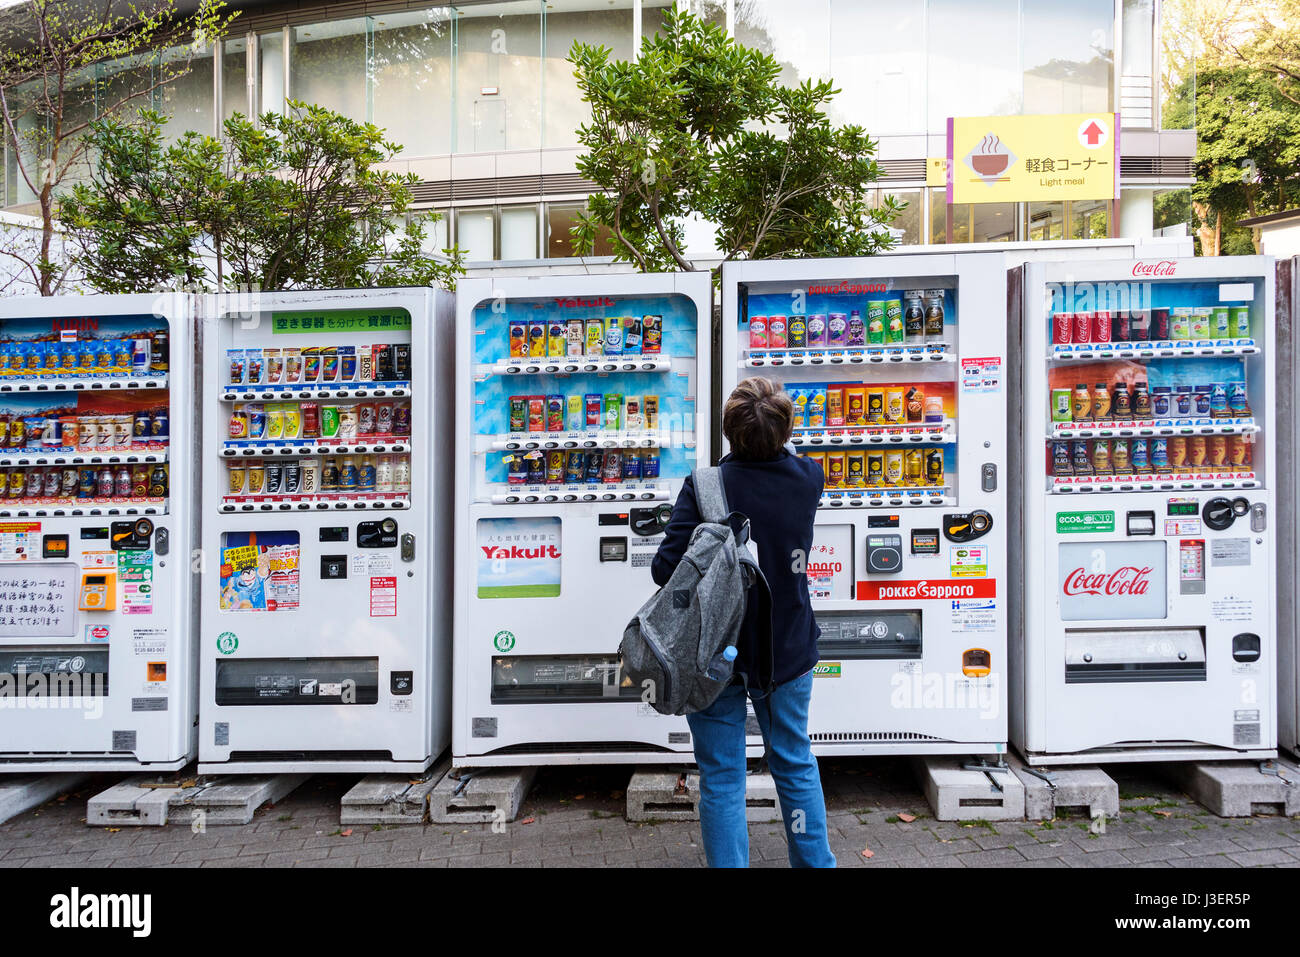
\includegraphics[scale = 0.5]{maquinaaescojer}
	\end{figure}
\end{frame}

\begin{frame}{Metodología}{(Continuación)}
	Estados (state).
	\begin{figure}
		
\includegraphics[scale = 0.5]{preguntas}
	\end{figure}
	\begin{equation}
		SD = \dfrac{100 \times T}{RT}
	\end{equation}
%Donde T es la duración en que la máquina falla y RT representa el tiempo total de procesamiento del resto de operaciones a partir de que la máquina falla. 
\end{frame}

\begin{frame}{Recompensa}
	``Entre más tiempo de espera menos es la recompensa"
	\begin{figure}
	\centering
	
\includegraphics[scale=0.15]{tiempodeespera}
	\end{figure} 
\end{frame}

\begin{frame}{Estructura}
	\begin{figure}
		\centering
		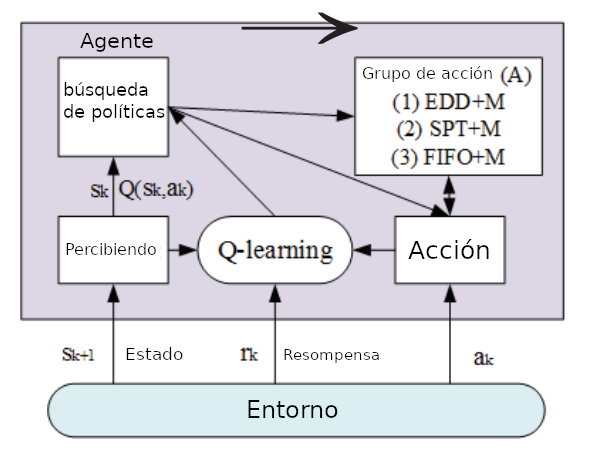
\includegraphics[scale=0.4]{estructura}
	\end{figure} 
\end{frame}

\begin{frame}{Algoritmo Genético \citep{batista2009}}
	\begin{figure}
		\centering
		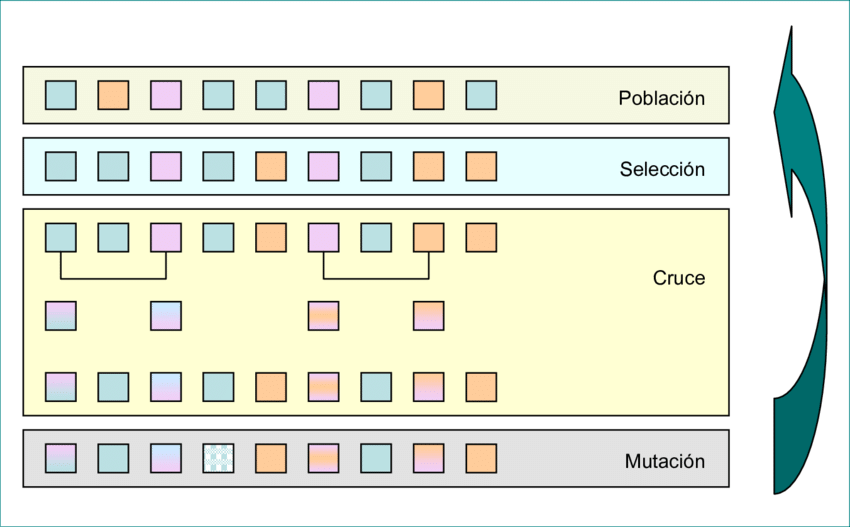
\includegraphics[scale = 0.35]{algoritmogenetico}
	\end{figure}
	%Se inicia con una planificación basada en GA programada en python del problema Mk03 que es un caso típico de programación de taller de trabajo flexible presentado por \cite{brandimarte1993routing} citado por \cite{zhao2019improved}. El parámetro de la población es de 50, el número de iteraciones es de 500, y las probabilidades transversal y de mutación son 0.8 y 0.2 respectivamente.
	
\end{frame}

\begin{frame}{Planificación con base en aprendizaje por refuerzo (Q-learning)}
Por ejemplo:
\setlength{\leftmargini}{60 pt}
\begin{enumerate}
	\item Ninguna
	\item SPT+M
	\item EDD+M
	\item FIFO+M
\end{enumerate}	
\end{frame}


{
\setbeamertemplate{background} 
{
    
\includegraphics[width=\paperwidth,height=\paperheight]{discussion.jpg}
}
\begin{frame}{Conclusiones}
\begin{enumerate}
	\item \fjssp
	\item tiempo
	\item resultados.
\end{enumerate}
%Hasta el momento en que se escribe esta propuesta, la evidencia bibliográfica indica que el uso de un aprendizaje por refuerzo en un \fjssp \, tiene resultados muy favorables; sin embargo esta propuesta también planea explorar el tiempo computacional de dicho aprendizaje el cual ya se mencionó puede explotar en ciertas circunstancias.

\end{frame}
}

\begin{frame}[allowframebreaks] %allow to expand references to multiple frames (slides)
	\frametitle{References}
	
	\bibliographystyle{apalike-es}
	\bibliography{bibliotarea1} %bibtex file name without .bib extension
	
\end{frame}


\end{document}
